\section{Auswertung}
\label{sec:Auswertung}

%Siehe \autoref{fig:plot}!
\subsection{Kontrast}

Zur Bestimmung des maximalen Kontrasts wurde der Winkel es Polaristionsfilters $\phi$ variiert und die jeweilige maximale und minimale Spannung in \autoref{tab:kontrast} notiert.
Daraus lässt sich über \autoref{eq:kontrast1} der Kontrast für jede Winkeleinstellung berechnen. 
\begin{table}
    \centering
    \caption{Winkeleinstellung des Polaristionsfilters $\phi$ und die entsprechenden maximalen und minimalen Spannungen an der Photodiode. Der daraus berechnete Kontrast $K$ ist ebenafalls aufgetragen.}
    \label{tab:kontrast}
    \begin{tabular}{c c c c}
        \toprule
        $\phi \,/\, \unit{\degree}$ & $I_\text{min} \,/\, \unit{\volt}$ & $I_\text{max} \,/\, \unit{\volt}$ & $K$ \\
        \midrule
        $0  $ &   $ 0.80\pm 0.01$ & $ 	0.99 \pm 0.01$ &  $ 0.11 \pm 0.01 $ \\
        $15	$ &   $ 0.48\pm 0.01$ & $	0.82 \pm 0.01$ &  $ 0.26 \pm 0.01 $ \\
        $30	$ &   $ 0.13\pm 0.01$ & $	0.77 \pm 0.01$ &  $ 0.71 \pm 0.02 $ \\
        $45	$ &   $ 0.10\pm 0.01$ & $	0.74 \pm 0.01$ &  $ 0.76 \pm 0.02 $ \\
        $50	$ &   $ 0.06\pm 0.01$ & $	0.84 \pm 0.01$ &  $ 0.87 \pm 0.02 $ \\
        $55	$ &   $ 0.04\pm 0.01$ & $	0.91 \pm 0.01$ &  $ 0.91 \pm 0.02 $ \\
        $60	$ &   $ 0.05\pm 0.01$ & $	0.97 \pm 0.01$ &  $ 0.90 \pm 0.02 $ \\
        $65	$ &   $ 0.09\pm 0.01$ & $	1.07 \pm 0.01$ &  $ 0.84 \pm 0.02 $ \\
        $80	$ &   $ 0.43\pm 0.01$ & $	1.20 \pm 0.01$ &  $ 0.47 \pm 0.01 $ \\
        $95	$ &   $ 0.92\pm 0.01$ & $	1.22 \pm 0.01$ &  $ 0.14 \pm 0.01 $ \\
        $110$ &   $ 0.54\pm 0.01$ & $  	1.95 \pm 0.01$ &  $ 0.57 \pm 0.01 $ \\
        $125$ &   $ 0.20\pm 0.01$ & $  	2.85 \pm 0.01$ &  $ 0.87 \pm 0.01 $ \\
        $130$ &   $ 0.15\pm 0.01$ & $  	3.00 \pm 0.01$ &  $ 0.90 \pm 0.01 $ \\
        $135$ &   $ 0.14\pm 0.01$ & $  	2.80 \pm 0.01$ &  $ 0.90 \pm 0.01 $ \\
        $140$ &   $ 0.14\pm 0.01$ & $  	2.89 \pm 0.01$ &  $ 0.91 \pm 0.01 $ \\
        $145$ &   $ 0.23\pm 0.01$ & $  	2.55 \pm 0.01$ &  $ 0.83 \pm 0.01 $ \\
        $160$ &   $ 0.56\pm 0.01$ & $  	2.16 \pm 0.01$ &  $ 0.59 \pm 0.01 $ \\
        $170$ &   $ 0.78\pm 0.01$ & $  	1.54 \pm 0.01$ &  $ 0.32 \pm 0.01 $ \\
        $180$ &   $ 0.81\pm 0.01$ & $  	1.01 \pm 0.01$ &  $ 0.11 \pm 0.01 $ \\
        \bottomrule
    \end{tabular}
\end{table}
Durch die Messwerte wird ein Fit der Form 
\begin{equation*}
    K(\phi) = A \cdot |\sin{\phi}\cos{\phi}|
\end{equation*}
gelegt.
Dabei ist $A$ der zu bestimmende Parameter.
Mit den Messwerten ergibt sich 
\begin{equation*}
    A = \qty{1.823(501)}{}
\end{equation*}
und der entsprechende Fit ist in \autoref{fig:kontrast} abgebildet.
\begin{figure}
    \centering
    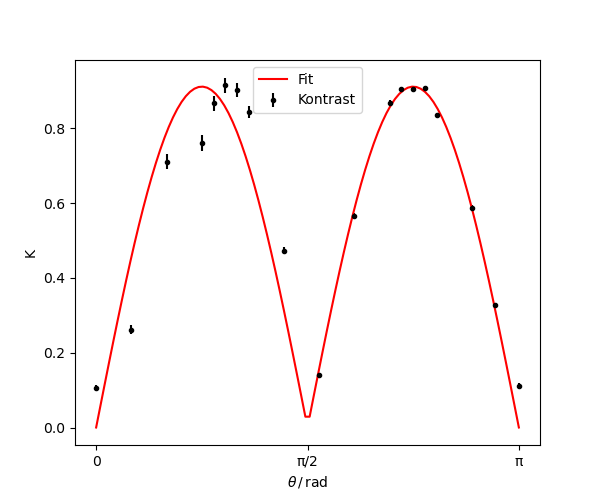
\includegraphics[width=0.9\textwidth]{python/kontrast.png}
    \caption{Fit der berechneten Kontraste in Abhängigkeit des Polaristionsfilter-Winkels.}
    \label{fig:kontrast}
\end{figure}

\subsection{Brechungsindex von Glas}
Die Anzahl der gemessenen Maxima $M$ bei Drehwinkel $\theta$ wurde insgesamt zehn mal durchgeführt.
Für jedes $M$ wird über \autoref{eq:n_glas} der Brechungsindex $n_\text{Luft}$ berechnet.
Das Ergebnis dieser Messreihen ist in \autoref{tab:glas} dargestellt.
\begin{table}
    \centering
    \caption{Anzahl gemessener Maxima $M$ und der daraus berechnete Brechungsindex $n_\text{Luft}$.}
    \label{tab:glas}
    \begin{tabular}{c c}
        \toprule
        $M$ & $n_\text{Luft}$ \\
        \midrule
        $32 \pm 1 $ & $1.498 \pm 0.023 $ \\
        $35 \pm 1 $ & $1.571 \pm 0.026 $ \\
        $33 \pm 1 $ & $1.522 \pm 0.024 $ \\
        $37 \pm 1 $ & $1.625 \pm 0.027 $ \\
        $32 \pm 1 $ & $1.498 \pm 0.023 $ \\
        $38 \pm 1 $ & $1.652 \pm 0.028 $ \\
        $29 \pm 1 $ & $1.431 \pm 0.021 $ \\
        $36 \pm 1 $ & $1.598 \pm 0.027 $ \\
        $34 \pm 1 $ & $1.546 \pm 0.025 $ \\
        $34 \pm 1 $ & $1.546 \pm 0.025 $ \\
        \bottomrule
    \end{tabular}
\end{table}
Über die so berechneten Brechungsindices wird gemittelt und somit ergibt sich als Endergebnis für den Brechungsindex von Luft
\begin{equation*}
    n_\text{Luft} = \qty{1.549(8)}{}.
\end{equation*}

\subsection{Brechungsindex von Luft}
Für jeden Druck $p$ wurden in je drei Messreihen die Anzahl Maxima $M$ bestimmt.
Außerdem wurde wie im vorherigen Abschnitt für jeden Messwert der Brechungsindex berechnet, dieses mal über \autoref{eq:n_luft}.
Das Ergebnis ist in \autoref{tab:brechung} niedergeschrieben.

\begin{table}
    \centering
    \caption{Brechungsindex $n$ in Abhängigkeit des Drucks $p$ in der Gaskammer und der Anzahl der Nulldurchgänge $M$ für drei Durchläufe.}
    \label{tab:brechung}
    \begin{tabular}{c c c c c c c}
        \toprule
        $p \,/\, \unit{\milli\pascal}$ & $M_1$ & $n_1$ & $M_2$ & $n_2$ & $M_3$ & $n_3$ \\
        \midrule
        $50	 $ &    $3.0\pm1.0	$ & $ 1.000019$ & $ 3.0\pm1.0  $ & $	1.000013$ & $3.0\pm1.0  $ & $ 1.000013$ \\
        $100 $ &    $5.0\pm1.0	$ & $ 1.000032$ & $ 5.0\pm1.0  $ & $	1.000025$ & $5.0\pm1.0  $ & $ 1.000025$ \\
        $150 $ &    $7.0\pm1.0	$ & $ 1.000044$ & $ 7.0\pm1.0  $ & $	1.000038$ & $7.0\pm1.0  $ & $ 1.000038$ \\
        $200 $ &    $9.0\pm1.0	$ & $ 1.000057$ & $ 9.0\pm1.0  $ & $	1.000057$ & $9.0\pm1.0  $ & $ 1.000051$ \\
        $250 $ &    $11.0\pm1.0 $ & $ 1.000070$ & $ 11.0\pm1.0 $ & $	1.000070$ & $11.0\pm1.0 $ & $ 1.000070$ \\
        $300 $ &    $13.0\pm1.0 $ & $ 1.000082$ & $ 13.0\pm1.0 $ & $	1.000082$ & $13.0\pm1.0 $ & $ 1.000082$ \\
        $350 $ &    $15.0\pm1.0 $ & $ 1.000095$ & $ 15.0\pm1.0 $ & $	1.000095$ & $15.0\pm1.0 $ & $ 1.000095$ \\
        $400 $ &    $17.0\pm1.0 $ & $ 1.000108$ & $ 17.0\pm1.0 $ & $	1.000108$ & $17.0\pm1.0 $ & $ 1.000108$ \\
        $450 $ &    $19.0\pm1.0 $ & $ 1.000120$ & $ 19.0\pm1.0 $ & $	1.000120$ & $19.0\pm1.0 $ & $ 1.000120$ \\
        $500 $ &    $21.0\pm1.0 $ & $ 1.000133$ & $ 21.0\pm1.0 $ & $	1.000133$ & $21.0\pm1.0 $ & $ 1.000133$ \\
        $550 $ &    $23.0\pm1.0 $ & $ 1.000146$ & $ 23.0\pm1.0 $ & $	1.000146$ & $23.0\pm1.0 $ & $ 1.000146$ \\
        $600 $ &    $25.0\pm1.0 $ & $ 1.000158$ & $ 25.0\pm1.0 $ & $	1.000158$ & $25.0\pm1.0 $ & $ 1.000158$ \\
        $650 $ &    $27.0\pm1.0 $ & $ 1.000171$ & $ 27.0\pm1.0 $ & $	1.000171$ & $27.0\pm1.0 $ & $ 1.000171$ \\
        $700 $ &    $30.0\pm1.0 $ & $ 1.000190$ & $ 30.0\pm1.0 $ & $	1.000190$ & $30.0\pm1.0 $ & $ 1.000190$ \\
        $750 $ &    $32.0\pm1.0 $ & $ 1.000203$ & $ 32.0\pm1.0 $ & $	1.000203$ & $32.0\pm1.0 $ & $ 1.000203$ \\
        $800 $ &    $34.0\pm1.0 $ & $ 1.000215$ & $ 34.0\pm1.0 $ & $	1.000215$ & $34.0\pm1.0 $ & $ 1.000215$ \\
        $850 $ &    $36.0\pm1.0 $ & $ 1.000228$ & $ 36.0\pm1.0 $ & $	1.000228$ & $36.0\pm1.0 $ & $ 1.000228$ \\
        $900 $ &    $38.0\pm1.0 $ & $ 1.000241$ & $ 38.0\pm1.0 $ & $	1.000247$ & $38.0\pm1.0 $ & $ 1.000241$ \\
        $950 $ &    $41.0\pm1.0 $ & $ 1.000260$ & $ 41.0\pm1.0 $ & $	1.000260$ & $41.0\pm1.0 $ & $ 1.000260$ \\
        $1000$ &	$42.0\pm1.0 $ & $ 1.000266$ & $ 42.0\pm1.0 $ & $	1.000266$ & $42.0\pm1.0 $ & $ 1.000266$ \\
        \bottomrule
    \end{tabular}
\end{table}
Für jeden der drei Messreihen wird entsprechend \autoref{eq:n_luft_lorentz} ein Fit der Form
\begin{equation*}
    n(p) = a \cdot \frac{p}{T R} + b 
\end{equation*}
durchgeführt.
Dabei ist $T = \qty{293.05}{\kelvin}$ die entsprechende Raumtemperatur und $R$ die allgemeine Gaskonstante.
